\documentclass[11pt,a4paper]{article}

\usepackage[margin=23mm]{geometry}
\usepackage{amsmath}
\usepackage{amssymb}
\usepackage{booktabs}
\usepackage{graphicx}
\usepackage{listings}
\usepackage{microtype}
\usepackage{siunitx}
\usepackage{tabularx}
\usepackage{tikz}
\usepackage[table]{xcolor}
\usepackage{xurl}
\usepackage[hidelinks]{hyperref}
\usepackage[section]{placeins}
\usetikzlibrary{arrows.meta,calc,positioning}

\sisetup{
  per-mode=symbol,
  range-phrase=--,
  range-units=single,
  table-number-alignment=center
}

\definecolor{primaryblue}{RGB}{31,95,145}
\definecolor{photonorange}{RGB}{210,105,30}
\definecolor{pairred}{RGB}{180,45,45}
\definecolor{meshgreen}{RGB}{48,130,89}
\definecolor{lightgray}{RGB}{245,246,248}

\newcommand{\vect}[1]{\boldsymbol{#1}}
\newcommand{\E}{\vect{E}}
\newcommand{\B}{\vect{B}}
\newcommand{\Pmom}{\vect{P}}
\newcommand{\betav}{\boldsymbol{\beta}}
\newcommand{\dd}{\mathrm{d}}
\newcommand{\code}[1]{\texttt{#1}}

\lstdefinestyle{commands}{
  basicstyle=\ttfamily\footnotesize,
  breaklines=true,
  breakatwhitespace=false,
  columns=fullflexible,
  frame=single,
  framerule=0.25pt,
  rulecolor=\color{black!35},
  backgroundcolor=\color{lightgray},
  keepspaces=true,
  showstringspaces=false,
  xleftmargin=1mm,
  xrightmargin=1mm
}

\title{Beam--Beam Fields and Passive Pair Tracking\\
       for a Gamma--Gamma Collider\\[4pt]
       \large Current OPALX Model and Validation Status}
\author{A. Adelmann}
\date{Draft of \today\\
      \small OPALX branch \code{271-implement-interation-point-element},
      commit \code{df7cd6cba}}

\begin{document}
\maketitle

\begin{abstract}
Low-energy electron--positron pairs created near the interaction point of a
gamma--gamma collider propagate through the collective electromagnetic fields
of the two primary electron bunches.  This note describes the current OPALX
model for that interaction, the CAIN input data, an independent manufactured
solution, and the present validation evidence.  The current implementation
supports exact timed witness emission, passive field sampling, a mirrored
primary source, single- and multi-GPU execution, and an optimized one-solve
field path.  A 12-particle benchmark agrees with the like-for-like
three-sigma-truncated manufactured trajectory to \SI{0.6004}{\percent} in the
transverse coordinate and \SI{0.0971}{\percent} longitudinally.  The remaining
work is dominated by the multiscale production mesh: a physical
\SI{15}{\centi\metre} aperture must coexist with a primary transverse rms size
of only \SI{1.944}{\micro\metre}.  A symmetric interaction window beginning
and ending at a primary-centroid distance $d=10\sigma_z$ from the interaction
point is proposed as the first cutoff-convergence hypothesis.
\end{abstract}

\section{Introduction and Problem Formulation}

The interaction region contains two counter-propagating high-energy electron
bunches, referred to here as the \emph{primary beams}.  Photons generated from
the primary beams collide close to the interaction point (IP) and produce
low-energy electron--positron pairs.  These particles are referred to as
\emph{witnesses}: they sample the primary collective field, but their number is
too small for their charge density or mutual interaction to be relevant in the
present model.  They therefore do not deposit charge and do not back-react on
the primaries.

The immediate objective is not pair generation inside OPALX.  Instead, CAIN
phase-space records are imported with an individual birth time for every
electron and positron.  OPALX must then transport each witness from its exact
birth event through the time-dependent fields of the two primary bunches.
The production target contains 1,297 electrons and 1,297 positrons.

Figure~\ref{fig:geometry} summarizes the model geometry.  The IP is the
midpoint of the placed \code{BEAMBEAM} element.  In the current production
geometry the element begins at $s=\SI{1}{\centi\metre}$, is
\SI{32}{\centi\metre} long, and therefore places the IP at
$s=\SI{17}{\centi\metre}$.  The second primary is represented by mirror
symmetry about the IP, not by a second independently tracked particle
container.

\begin{figure}[htbp]
  \centering
  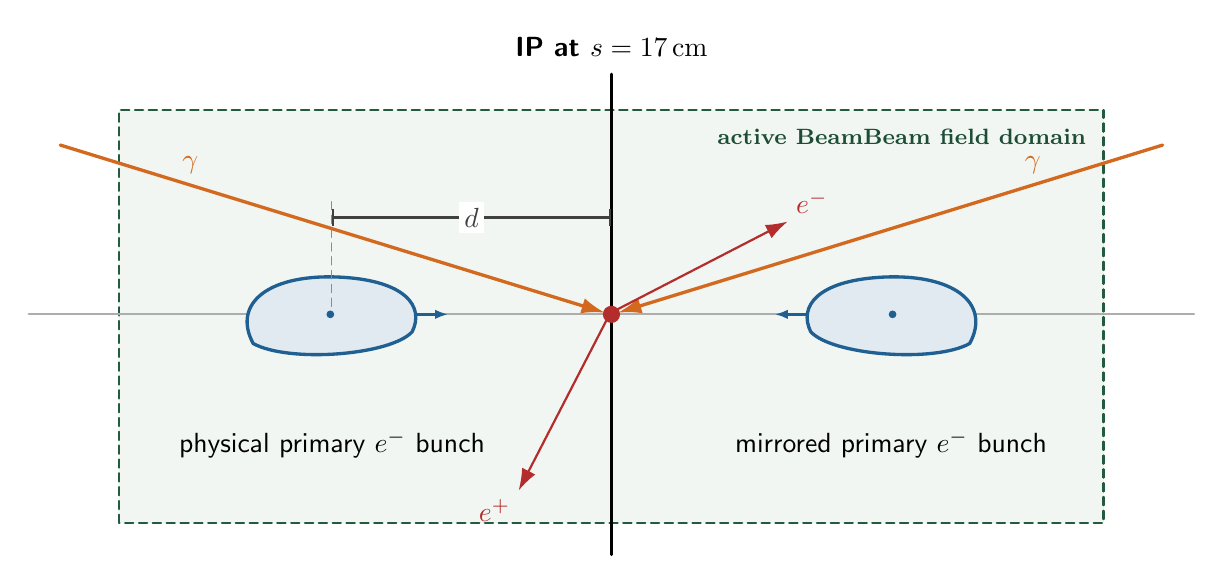
\begin{tikzpicture}[
      >=Latex,
      line cap=round,
      line join=round,
      font=\sffamily,
      primary/.style={draw=primaryblue, fill=primaryblue!13, very thick},
      primary arrow/.style={primaryblue, very thick,
                            -{Latex[length=1.7mm,width=1.2mm]}},
      photon/.style={photonorange, very thick,
                     -{Latex[length=3.0mm,width=2.0mm]}},
      pair arrow/.style={pairred, thick,
                         -{Latex[length=2.8mm,width=1.9mm]}},
      label text/.style={align=center, text=black}
  ]
    \fill[meshgreen!7] (-6.25,-2.65) rectangle (6.25,2.60);
    \draw[meshgreen!70!black, densely dashed, thick]
      (-6.25,-2.65) rectangle (6.25,2.60);
    \node[meshgreen!60!black, anchor=north east, font=\footnotesize\bfseries]
      at (6.15,2.48) {active BeamBeam field domain};

    \draw[black!32, thick] (-7.4,0) -- (7.4,0);
    \draw[black, very thick] (0,-3.05) -- (0,3.05);
    \node[font=\sffamily\bfseries, above=3pt] at (0,3.05)
      {IP at $s=\SI{17}{\centi\metre}$};

    \begin{scope}[shift={(-3.55,0.05)}]
      \draw[primary] (-1.00,-0.42)
        .. controls (-1.28,0.10) and (-0.78,0.48) .. (0.15,0.42)
        .. controls (0.92,0.37) and (1.18,0.06) .. (1.02,-0.27)
        .. controls (0.75,-0.57) and (-0.55,-0.67) .. cycle;
      \fill[primaryblue] (-0.02,-0.05) circle (1.4pt);
    \end{scope}
    \node[label text, below=7pt] at (-3.55,-1.10)
      {physical primary $e^-$ bunch};

    \begin{scope}[shift={(3.55,0.05)},xscale=-1]
      \draw[primary] (-1.00,-0.42)
        .. controls (-1.28,0.10) and (-0.78,0.48) .. (0.15,0.42)
        .. controls (0.92,0.37) and (1.18,0.06) .. (1.02,-0.27)
        .. controls (0.75,-0.57) and (-0.55,-0.67) .. cycle;
      \fill[primaryblue] (-0.02,-0.05) circle (1.4pt);
    \end{scope}
    \node[label text, below=7pt] at (3.55,-1.10)
      {mirrored primary $e^-$ bunch};

    % Exactly 4 mm long at the native TikZ scale, beginning at the inward edges.
    \draw[primary arrow] (-2.47,0) -- ++(0.40,0);
    \draw[primary arrow] ( 2.47,0) -- ++(-0.40,0);

    \draw[black!75, thick, |-|] (-3.55,1.23) -- (0,1.23)
      node[midway, fill=white, inner sep=2pt] {$d$};
    \draw[black!45, densely dashed] (-3.55,0.10) -- (-3.55,1.43);

    \draw[photon] (-7.0,2.15) -- (-0.08,0.02);
    \draw[photon] ( 7.0,2.15) -- ( 0.08,0.02);
    \node[photonorange, font=\sffamily\bfseries, above]
      at (-5.35,1.66) {$\gamma$};
    \node[photonorange, font=\sffamily\bfseries, above]
      at (5.35,1.66) {$\gamma$};

    \fill[pairred] (0,0) circle (3.1pt);
    \draw[pair arrow] (0.05,0.05) -- (2.24,1.18)
      node[above right=-1pt,text=pairred,font=\sffamily\bfseries] {$e^-$};
    \draw[pair arrow] (-0.05,-0.05) -- (-1.18,-2.24)
      node[below left=-1pt,text=pairred,font=\sffamily\bfseries] {$e^+$};
  \end{tikzpicture}
  \caption{Beam--beam geometry.  The primary and mirrored-primary centroids
  approach the IP from opposite sides.  The distance $d$ is defined from one
  primary centroid to the IP; the centroid-to-centroid separation is $2d$.
  Witness particles are released at their individual birth times and sample
  the primary fields without contributing to the field solve.}
  \label{fig:geometry}
\end{figure}

The reference primary parameters are collected in
Table~\ref{tab:primary-parameters}.  The primary support used for controlled
manufactured comparisons is truncated independently in each coordinate at
three rms sizes and renormalized.

\begin{table}[htbp]
  \centering
  \caption{Reference primary and production interaction-region parameters.}
  \label{tab:primary-parameters}
  \begin{tabular}{@{}lll@{}}
    \toprule
    Quantity & Symbol or input & Value \\
    \midrule
    Primary kinetic energy & $K_0$ & \SI{245}{\mega\electronvolt} \\
    Electrons per primary bunch & $N_e$ & $1.25\times10^{10}$ \\
    Transverse rms size & $\sigma_x=\sigma_y$ & \SI{1.944325075701}{\micro\metre} \\
    Longitudinal rms size & $\sigma_z$ & \SI{0.6}{\milli\metre} \\
    Controlled source support & & $|x_i|\leq3\sigma_i$ \\
    Production element length & $L_{\mathrm{BB}}$ & \SI{32}{\centi\metre} \\
    Production aperture radius & $R_{\mathrm{ap}}$ & \SI{15}{\centi\metre} \\
    Production witnesses & & $1297~e^-+1297~e^+$ \\
    \bottomrule
  \end{tabular}
\end{table}

For a witness of charge $q$ and mass $m_e$, OPALX uses normalized momentum
$\Pmom=\gamma\betav$.  The continuous equations represented by the particle
pusher are
\begin{align}
  \frac{\dd\vect x}{\dd t}
    &= c\frac{\Pmom}{\sqrt{1+\Pmom^2}}, \\
  \frac{\dd\Pmom}{\dd t}
    &= \frac{q}{m_e c}
       \left(\E+c\frac{\Pmom}{\sqrt{1+\Pmom^2}}\times\B\right).
\end{align}
The fields are the superposition of the physical and mirrored primary
contributions.  Witness fields are excluded.

\section{CAIN Results}

CAIN supplies two datasets with complementary roles.  The file
\code{fort98.txt} contains the production population of 1,297 electrons and
1,297 positrons.  The artificial Track-12 dataset contains six
electron--positron pairs and densely sampled trajectories used for exact-timed
code-to-code comparison.

In the converted production data, paired electrons and positrons have identical
creation coordinates and creation times.  Their momenta differ according to
the pair kinematics.  The creation times span
\SIrange{-4.137532}{3.237053}{\pico\second}, have a standard deviation of
\SI{1.037166}{\pico\second}, and are equal within each electron--positron pair.
The mean kinetic energies are \SI{313.60}{\kilo\electronvolt} for both species.
The momentum directions are broad: approximately half of each species travels
with positive $p_z$ and half with negative $p_z$.

\begin{figure}[htbp]
  \centering
  \includegraphics[width=0.90\textwidth]
    {../track-e-p/data/pair_momentum_time_histogram.png}
  \caption{CAIN production-pair creation-time distribution.  The upper panel
  shows the identical electron and positron time spectra; the lower panel
  verifies zero pair-wise time difference for all 1,297 pairs.}
  \label{fig:cain-times}
\end{figure}

\begin{figure}[htbp]
  \centering
  \includegraphics[width=0.92\textwidth]
    {../track-e-p/data/pair_momentum_directions.png}
  \caption{Direction distributions of the CAIN production witnesses.  The
  broad angular support is important for the field-mesh coverage and aperture
  studies: the witness population is not a narrow paraxial beam.}
  \label{fig:cain-directions}
\end{figure}

The Track-12 births occur at
\begin{equation}
  ct = (-0.9000,-0.5994,-0.3006,0,0.3006,0.5994)\ \si{\milli\metre}.
\end{equation}
CAIN samples every
\begin{equation}
  \Delta t = \frac{\SI{1.8}{\micro\metre}}{c}
           = \SI{6.004153713566736}{\femto\second}
\end{equation}
through $ct=\SI{1.8}{\milli\metre}$.  OPALX uses the same clock, so all 13,012
trajectory samples can be compared without temporal interpolation.

CAIN and the current OPALX manufactured model do not use identical collective
field descriptions.  CAIN is therefore a physics comparison, not the numerical
oracle for the OPALX Poisson solve.  Agreement with CAIN and agreement with the
like-for-like manufactured solution must be reported separately.

\section{Manufactured Solution}

The independent manufactured solution represents two unchanging, uniformly
moving anisotropic Gaussian primary bunches.  Their centroids move in opposite
longitudinal directions, and the IP is at the origin.  For a source moving with
velocity $\vect v_s=c\betav_s$, the laboratory-frame event is transformed to
the source rest frame.  In the present straight geometry,
\begin{equation}
  x'=x-x_c(t),\qquad
  y'=y-y_c(t),\qquad
  z'=\gamma_s[z-z_c(t)].
\end{equation}
The rest-frame rms sizes are
\begin{equation}
  \sigma_x'=\sigma_x,\qquad
  \sigma_y'=\sigma_y,\qquad
  \sigma_z'=\gamma_s\sigma_z.
\end{equation}

For an untruncated triaxial Gaussian, the rest-frame electric field is evaluated
with the ellipsoidal integral
\begin{equation}
 E_i'(\vect r') =
 \frac{Qx_i'}{4\pi\epsilon_0\sqrt{2\pi}}
 \int_0^\infty
 \frac{\exp\!\left[-\frac{1}{2}\sum_j
       \frac{x_j'^2}{\sigma_j'^2+u}\right]}
 {(\sigma_i'^2+u)
  \sqrt{(\sigma_x'^2+u)(\sigma_y'^2+u)(\sigma_z'^2+u)}}\,\dd u .
\end{equation}
The independent evaluator uses logarithmic quadrature in $u$, which resolves
the large rest-frame aspect ratio.  With $\B'=0$, the laboratory fields are
obtained from the uniform-motion Lorentz transformation.  For a boost along
$z$,
\begin{equation}
  E_x=\gamma_s E_x',\qquad E_y=\gamma_s E_y',\qquad E_z=E_z',
  \qquad
  \B=\frac{1}{c^2}\vect v_s\times\E.
\end{equation}

Like-for-like OPALX comparisons use a component-wise three-sigma-truncated and
renormalized density.  This removes finite-support mismatch while retaining an
independent field evaluator.  At a three-$\sigma_z$ centroid separation, a
20,301-probe comparison gave the results in
Table~\ref{tab:three-sigma-field}.

\begin{table}[htbp]
  \centering
  \caption{Three-$\sigma_z$ physical-plus-mirrored manufactured-field
  comparison.}
  \label{tab:three-sigma-field}
  \begin{tabular}{@{}lr@{}}
    \toprule
    Quantity & Value \\
    \midrule
    OPALX maximum $|\E|$ & $5.545751\times10^9\ \si{\volt\per\metre}$ \\
    Manufactured maximum $|\E|$ & $5.553866\times10^9\ \si{\volt\per\metre}$ \\
    Relative $L_2$ error, $\E$ & \SI{1.1098}{\percent} \\
    Median field-magnitude ratio & 0.997923 \\
    Median direction cosine & 0.999970 \\
    Relative $L_2$ error, $\B$ & \SI{1.1098}{\percent} \\
    \bottomrule
  \end{tabular}
\end{table}

At exact centroid overlap, the identical sources have equal electric fields and
opposite magnetic fields.  The manufactured solution therefore predicts exact
magnetic cancellation.  The corresponding focused C++ regression verifies
doubled deposited charge, restored physical coordinates, doubled electric
field for a mirror-symmetric source, and cancelled magnetic field on one and
two MPI ranks.

\begin{figure}[htbp]
  \centering
  \includegraphics[width=0.92\textwidth]{../reduced-order-model/outputs/comparison-two-source/3sigma_physical_and_copied_field_comparison.png}
  \caption{Representative three-$\sigma_z$ comparison of the OPALX
  physical-plus-mirrored field with the independent anisotropic Gaussian
  manufactured solution.}
  \label{fig:manufactured-field}
\end{figure}

\section{Current OPALX Model}

\subsection{Software architecture}

The status described here corresponds to branch
\texttt{271-implement-interation-\allowbreak point-element} at commit
\code{df7cd6cba}.  The
seven-step element redesign is complete.  \code{BeamBeam} now follows the same
ownership model as ordinary OPALX elements: the placed element contains input
and placement configuration, while mutable per-run state belongs to
\code{BeamBeamInteraction}.  A generic \code{ElementInteractionManager} owns
the interaction, and \code{ParallelTracker} dispatches generic
\code{SelfField}, \code{AfterEmission}, and \code{Diagnostics} phases.  The
tracker no longer contains a BeamBeam-specific branch.

The IP is unconditionally the midpoint of the placed element.  The former
\code{IP\_S} override has been removed.  The current one-bin, no-cathode path
uses only the persistent fields $\E_m$ and $\B_m$:
\begin{equation*}
\begin{split}
  \text{primary particles}
  &\longrightarrow \rho
  \longrightarrow \text{one open-boundary Poisson solve}
  \longrightarrow (\E_p,\B_p) \\
  &\longrightarrow \text{reflection about the IP}
  \longrightarrow (\E_v,\B_v) \\
  &\longrightarrow (\E_m,\B_m)=(\E_p+\E_v,\B_p+\B_v).
\end{split}
\end{equation*}
Reflection and accumulation execute in the active Kokkos memory space.  The
full fields are not staged through host memory.  This path reduced ten-step
solver calls from 20 to 11, where the remaining extra solve is warm-up, and
reduced measured BeamBeam self-field time by \SI{45.2}{\percent}.

\subsection{Particle and emission contract}

The three-container contract is
\begin{center}
\begin{tabular}{@{}cll@{}}
  \toprule
  Container & Particles & Field role \\
  \midrule
  0 & primary electrons & deposits charge and normally receives the field \\
  1 & CAIN electrons & passive gather only \\
  2 & CAIN positrons & passive gather only \\
  \bottomrule
\end{tabular}
\end{center}
The \code{BBRIGID=TRUE} option suppresses the BeamBeam collective kick only on
container 0.  It does not suppress deposition, witness gathering, ordinary
drift, or external fields.  It is used for controlled comparison with the
rigid manufactured source; production defaults to \code{BBRIGID=FALSE}.

Timed emitted files store
\begin{center}
  \code{x y z px py pz birth\_time}.
\end{center}
The momentum components are $p/(m_ec)$ and the positions are relative to the
emission-source origin.  A witness born inside a step is integrated only over
the fractional interval
\begin{equation}
  \Delta t_{\mathrm{particle}}=t_{\mathrm{step\ end}}-t_{\mathrm{birth}}.
\end{equation}
Before gathering, each witness position is transformed from its independent
container reference frame to the source-field frame.  The gather then performs
an MPI owner-rank reduction and transforms the sampled fields back.

\subsection{Current fixed mesh and its limitation}

During BeamBeam activity the field mesh is fixed to
\begin{equation}
 x\in[-a_x,a_x],\qquad y\in[-a_y,a_y],\qquad
 z\in[z_{\mathrm{IP}}-L/2,z_{\mathrm{IP}}+L/2].
\end{equation}
For the production geometry this is a rectangular box of
$\SI{30}{\centi\metre}\times\SI{30}{\centi\metre}\times
\SI{32}{\centi\metre}$ enclosing the cylindrical aperture.  The implementation
currently checks only the transverse extent of container 0.  It does not prove
containment of the mirrored source or witness containers, and it does not check
longitudinal containment.

More importantly, geometric coverage is not numerical resolution.  The
current large-cylinder debug deck uses $16^3$ cells, corresponding to cell
sizes of approximately \SI{20}{\milli\metre}, \SI{20}{\milli\metre}, and
\SI{21.33}{\milli\metre}.  Even a $4096\times256\times128$ mesh over the same
box would have spacings of approximately \SI{73.3}{\micro\metre},
\SI{1.176}{\milli\metre}, and \SI{2.52}{\milli\metre}; it would not resolve the
\SI{1.944}{\micro\metre} transverse primary or the \SI{0.6}{\milli\metre}
longitudinal primary.  The physical aperture and numerical field domain must
therefore be separated.

\section{Current OPALX Results}

The current validation hierarchy is summarized in
Table~\ref{tab:validation}.  The complete local build and focused tests pass;
Kokkos version 5.2.0 is configured.  MPI-sensitive paths have been exercised
on one, two, and four ranks.

\begin{table}[htbp]
  \centering
  \caption{Selected validation and performance evidence.}
  \label{tab:validation}
  \small
  \begin{tabularx}{\textwidth}{@{}p{28mm}p{25mm}p{22mm}Xr@{}}
    \toprule
    Test & Particles & Mesh & Result & Wall time \\
    \midrule
    Persistent manufactured CTest
      & 100,000 source; 5,151 probes
      & $64\times64\times128$
      & Relative $L_2(\E,\B)=(2.10,2.20)\%$
      & $\sim\SI{5}{\second}$ \\
    Fixed-source rank scan
      & 400,000 source; 5,151 probes
      & $64\times64\times128$
      & Four-rank fields agree with one rank to $2.4\times10^{-16}$
      & \SIrange{4.94}{10.50}{\second} \\
    Witness-gather rank regression
      & 100,000 source; $8e^-+8e^+$
      & $32\times32\times64$
      & Rank differences in field and kick below $1.5\times10^{-15}$
      & \SIrange{5.85}{9.82}{\second} \\
    Fine Track-12, four A100s
      & 400,000 source; $6e^-+6e^+$
      & $4096\times256\times128$
      & 1,501 steps; all 13,012 samples; normal completion
      & \SI{25278.83}{\second} \\
    \bottomrule
  \end{tabularx}
\end{table}

The transverse first-kick refinement keeps the field domain fixed at
\SI{2.4}{\milli\metre} by \SI{0.24}{\milli\metre} and $N_z=128$.  Refinement
changes the field magnitude while the direction cosine remains at least
0.999993.  The observed trend approaches second order, but anisotropic
refinement matters: increasing $N_x$ while coarsening $N_y$ does not guarantee
a smaller error.

\begin{figure}[htbp]
  \centering
  \includegraphics[width=0.96\textwidth]{../track12particles/opalx/timed/a100_mesh_8da5b9e83_1rank/pair4_field_and_kick_convergence.png}
  \caption{Pair-4 electric-field and first-kick convergence toward the
  three-sigma-truncated manufactured source.  The first three coarse points and
  last four fine points are fitted separately.}
  \label{fig:mesh-convergence}
\end{figure}

For the full $4096\times256\times128$, 1,501-step trajectory, the principal
comparison is
\begin{center}
\begin{tabular}{@{}lrrrr@{}}
  \toprule
  Reference & $x$ relative $L_2$ & $x$ RMSE
            & longitudinal relative $L_2$ & longitudinal RMSE \\
  \midrule
  Manufactured & \SI{0.6004}{\percent} & \SI{1.996}{\micro\metre}
               & \SI{0.0971}{\percent} & \SI{0.807}{\micro\metre} \\
  CAIN & \SI{9.545}{\percent} & \SI{30.648}{\micro\metre}
       & \SI{2.9774}{\percent} & \SI{24.477}{\micro\metre} \\
  \bottomrule
\end{tabular}
\end{center}
The twelve first-$x$-kick ratios relative to the truncated manufactured model
span 0.92947--0.97490, with mean 0.94860.  Charge-conjugate OPALX kicks agree to
a maximum relative residual of $7.57\times10^{-10}$.  This supports the timed
input, species assignment, charge sign, MPI gather, and fractional integration.
The larger CAIN discrepancy is attributed to a difference in collective source
model or convention and must not be tuned away in OPALX.

\begin{figure}[htbp]
  \centering
  \includegraphics[width=\textwidth]{../track12particles/opalx/timed/a100_4rank_400k_4096x256x128_twofield_816d11ff8/results/track12_cain_vs_opalx.png}
  \caption{Latest four-A100 Track-12 comparison.  CAIN is shown at left, OPALX
  with exact timed births in the centre, and the three-sigma-truncated rigid
  two-Gaussian manufactured solution at right.}
  \label{fig:track12}
\end{figure}

The optimized two-field result changes the previous two-solve trajectory only
at accumulated numerical levels: the maximum position changes are below
\SI{0.022}{\micro\metre}, and relative $L_2$ momentum differences are below
$4\times10^{-6}$.  The optimized full trajectory is 1.992 times faster than
the otherwise identical two-solve run.

\section{Next Steps in Refining the OPALX Model}

\subsection{Define a physical interaction cutoff}

The first hypothesis is a symmetric interaction window defined by the distance
of either primary centroid from the IP,
\begin{equation}
  d=10\sigma_z=\SI{6}{\milli\metre}.
\end{equation}
With the 245 MeV primary, $\beta=0.999997834$, so
\begin{equation}
  \frac{d}{\beta c}=\SI{20.0}{\pico\second}.
\end{equation}
The mirrored interaction would begin approximately \SI{20}{\pico\second}
before centroid overlap and end approximately \SI{20}{\pico\second} after it.
At activation the centroid separation is $2d=\SI{12}{\milli\metre}$.  A
three-sigma-truncated source has its nearest edge seven rms lengths from the
IP.

This is a cutoff hypothesis, not an accuracy result.  Gaussian density at the
IP is exponentially small at ten rms lengths, but the electromagnetic field is
long-ranged.  The integrated witness and primary impulses must be converged for
$d/\sigma_z=5,7.5,10,15,$ and 20.  The comparison quantities should include
final position and momentum, maximum transverse kick, primary moments at the
IP, and aperture-loss count and location.

The implementation semantics also require refinement.  Before the symmetric
window the physical primary may continue its ordinary self-field evolution.
Inside it, the physical and mirrored fields are combined and gathered to the
witnesses.  After it, the mirrored BeamBeam contribution and witness gather are
disabled.  This is not identical to the current \code{COPY\_TIME}, which only
enables the mirror, or \code{RETIRE\_TIME}, which deletes the physical source.
A geometric interaction-distance parameter is preferable to two absolute
times tied to the upstream tracking origin.

\subsection{Separate physical and numerical domains}

For $d=10\sigma_z$ and a three-sigma source, the longitudinal numerical domain
must satisfy
\begin{equation}
  z_{\mathrm{half}}\gtrsim d+3\sigma_z
  =13\sigma_z=\SI{7.8}{\milli\metre},
\end{equation}
plus a mesh and interpolation margin.  This suggests a numerical field length
of approximately \SIrange{16}{18}{\milli\metre}, not the full
\SI{32}{\centi\metre} physical element.

The next code-level diagnostic should compute global minimum and maximum
positions for all active containers in the source-field frame on every
BeamBeam solve.  It should report the distance to each field boundary in metres
and cells and fail clearly when a source or gathered witness lies outside the
supported interpolation region.  The current primary-only transverse check is
insufficient.

The transverse scale separation remains harder.  A witness may move several
millimetres during a \SI{40}{\pico\second} interaction window, whereas the
primary transverse rms size is only \SI{1.944}{\micro\metre}.  A single uniform
mesh that covers both scales and resolves the primary with several cells per
rms size is expensive.  Candidate refinements are a compact source mesh with a
separate far-field evaluator, nested meshes, or a controlled analytic rigid
Gaussian field outside the resolved source region.  Each option must preserve
the non-rigid production path and be validated against the manufactured
solution.

\clearpage
\subsection{Production-readiness sequence}

Before interpreting a full 1,297-pair production run, the following sequence is
required:
\begin{enumerate}
  \item Align the timed CAIN file origin with the primary centroid-overlap
        clock and migrate the large-cylinder input from common-\code{T0}
        \code{FROMFILE} injection to the exact timed files.
  \item Add source, mirror, and witness mesh-coverage diagnostics and a
        regression for out-of-domain gathering.
  \item Decouple physical element length and aperture from the numerical field
        domain.
  \item Converge the interaction cutoff $d$, timestep, transverse and
        longitudinal mesh, primary macroparticle count, and source truncation.
  \item Repeat the selected production case on one and multiple A100s and
        verify decomposition independence of fields, trajectories, and losses.
  \item Correct the known H5 electric-field unit metadata, which currently
        labels values stored in \si{\volt\per\metre} as \si{\mega\volt\per\metre},
        after auditing downstream readers.
\end{enumerate}

The first complete production run should therefore be treated as a workflow
and coverage test.  Physics conclusions about pair losses should be drawn only
after the cutoff and discretization studies are complete.

\clearpage
\appendix
\section{Reproducing the Data, Figures, and OPALX Runs}
\label{app:reproduction}

This appendix records the workflow used for the results in this note.  Unless
stated otherwise, commands are run from the root of the
\code{opalx-beambeam} checkout with the Python environment
\code{\$HOME/.venv-h6}.  Generated H5 files and plots are intentionally ignored
by Git.  A reproducible run must retain the Git revision, input hashes, mesh,
timestep, particle count, MPI rank count, GPU identity, executable hash,
\code{runtime\_compute.txt}, nonempty \code{timing.dat}, and the scheduler log.

The results reported here correspond to the source state identified in
Section~4.1.  To reproduce a historical number exactly, check out that
revision and do not reuse input or manifest files from a different mesh.  For
new studies, use the current branch tip and record the resulting revision in
the run manifest.

\subsection{Figure provenance}

Table~\ref{tab:figure-provenance} maps every figure in this note to its source
or generating program.  Figure~\ref{fig:geometry} is native TikZ in this
\LaTeX{} file and is regenerated by compiling the note.

\begin{table}[htbp]
  \centering
  \caption{Programs and principal output files for the figures in this note.}
  \label{tab:figure-provenance}
  \small
  \begin{tabularx}{\textwidth}{@{}p{12mm}p{44mm}X@{}}
    \toprule
    Figure & Program or source & Output used by this note \\
    \midrule
    \ref{fig:geometry} & \code{bb-note.tex}
      & inline TikZ, generated during \LaTeX{} compilation \\
    \ref{fig:cain-times} & \code{analyze\_pair\_momenta.py}
      & \path{pair_momentum_time_histogram.png} \\
    \ref{fig:cain-directions} & \code{analyze\_pair\_momenta.py}
      & \path{pair_momentum_directions.png} \\
    \ref{fig:manufactured-field}
      & \code{compare\_opalx\_fields.py}
      & \path{3sigma_physical_and_copied_field_comparison.png} \\
    \ref{fig:mesh-convergence}
      & \code{scan\_first\_kick\_fields.py}
      & \path{pair4_field_and_kick_convergence.png} \\
    \ref{fig:track12}
      & \code{compare\_timed\_track12.py}
      & \path{results/track12_cain_vs_opalx.png} \\
    \bottomrule
  \end{tabularx}
\end{table}

\subsection{CAIN pair data and Figures~\ref{fig:cain-times}--\ref{fig:cain-directions}}

The full CAIN pair table is \code{sandbox/track-e-p/fort98.txt}.  Convert it to
separate OPALX electron and positron files while retaining the individual
creation times, then make the statistical tables and figures as follows:

\begin{lstlisting}[style=commands]
cd sandbox/track-e-p
$HOME/.venv-h6/bin/python convert_fort98_to_fromfile.py \
  fort98.txt --add-time -o .
$HOME/.venv-h6/bin/python analyze_pair_momenta.py \
  --electron-file gamma_gamma_electrons-t.fromfile \
  --positron-file gamma_gamma_positrons-t.fromfile \
  --output-dir data --plot
cd ../..
\end{lstlisting}

The second command writes the two PNG files used in this note, CSV summaries, a
representative pair-geometry plot, and a multipage PDF.  Species pairing is by
row order from the CAIN event table; the conversion should therefore be rerun
whenever \code{fort98.txt} changes.

\clearpage
\subsection{Independent manufactured solution}

The independent field evaluator implements the Lorentz transformation of an
anisotropic Gaussian at uniform velocity.  It does not call the OPALX field
solver.  Generate the smooth field snapshots at centroid separations
$d/\sigma_z=3,2,1,0$ and run its focused tests with

\begin{lstlisting}[style=commands]
$HOME/.venv-h6/bin/python \
  sandbox/reduced-order-model/python/rigid_two_gaussian_fields.py
$HOME/.venv-h6/bin/python -m unittest \
  sandbox/reduced-order-model/python/test_rigid_two_gaussian_fields.py \
  sandbox/reduced-order-model/python/test_fixed_primary_fromfile.py
\end{lstlisting}

Within \code{sandbox/reduced-order-model}, the field tables, summary JSON, and
overview plot are written below \path{outputs/fields}; the authoritative inputs
are in \path{parameters.json}.  Electric fields are
in \si{\volt\per\metre}, magnetic fields in tesla, positions in metres, and
momenta in $m_ec$ units.

For the OPALX comparison in Figure~\ref{fig:manufactured-field}, first generate
and run the matching OPALX probe cases locally, then compare the two-source
field after mirroring:

\begin{lstlisting}[style=commands]
$HOME/.venv-h6/bin/python \
  sandbox/reduced-order-model/python/make_opalx_field_cases.py --run
$HOME/.venv-h6/bin/python \
  sandbox/reduced-order-model/python/compare_opalx_fields.py \
  --cases 3sigma --step 1 \
  --source-model physical-and-copied \
  --output-dir \
    sandbox/reduced-order-model/outputs/comparison-two-source
\end{lstlisting}

The default generator uses 400,000 primary macroparticles, a
$64\times64\times128$ field mesh, and a $101\times201$ passive-probe grid.  The
odd probe dimensions place a sample exactly at the IP.  \code{Step\#0} is the
physical bunch alone; \code{Step\#1} is the physical-plus-mirrored field.  The
OPALX deck must use \code{GREENSF=INTEGRATED}, \code{BBRIGID=TRUE}, and
\code{EBDUMP=TRUE} for this comparison.

The manufactured Track-12 trajectories are recomputed by
\code{compare\_timed\_track12.py}; they are not read from a stored trajectory.
The integrator uses both anisotropic sources, component-wise three-sigma source
truncation, exact CAIN birth times, and a maximum internal substep of
\SI{1}{\femto\second}.

\subsection{Building OPALX for Merlin6}

The GPU calculations use the persistent Merlin6 checkout and its configured
Release build.  Login-node availability can be intermittent, so all expensive
work is submitted through Slurm and all scripts and logs are stored inside the
run directory.  On Merlin6:

\begin{lstlisting}[style=commands]
ssh merlin6
SRC=/psi/home/adelmann/opalx-dev/opalx-a100-5a354101f
cd "$SRC"
git status --short
git rev-parse HEAD
cmake --build build-a100 -j20
grep CMAKE_BUILD_TYPE build-a100/CMakeCache.txt
OPALX="$SRC/build-a100/src/opalx"
test -x "$OPALX"
\end{lstlisting}

The intended configuration is Release with CUDA and Ampere-80 support.  If the
existing build directory is unavailable, it must be configured with the
Merlin site dependency prefixes before the build command above; those paths
are installation-specific and should not be guessed.  Record the CMake cache
and \code{sha256sum \$OPALX} in a fresh production campaign.

\clearpage
\subsection{Manufactured-field A100 study on Merlin6}

The self-submitting convergence driver prepares its input matrix, launches the
single-GPU cases, then connected two- and four-rank MPI cases, and finally
checks completion.  It copies scheduler output into \code{RUN\_ROOT/slurm}.

\begin{lstlisting}[style=commands]
cd "$SRC"
RUN_ROOT=/psi/home/adelmann/opalx-dev/\
bb-manufactured-$(git rev-parse --short HEAD)-$(date -u +%Y%m%dT%H%M%SZ)
sandbox/reduced-order-model/merlin/submit_a100_convergence.sh \
  --run-root "$RUN_ROOT" --repo-root "$SRC" --opalx "$OPALX"
squeue -M gmerlin6
\end{lstlisting}

Connected multi-GPU runs use \code{mpiexec} with one rank per A100 and
\path{--kokkos-map-device-id-by=mpi_rank}.  Plain multi-task \code{srun} must
not launch OPALX on this cluster because it creates independent Open MPI
singletons.  Independent one-rank cases may run as exclusive \code{srun} steps
inside a GPU allocation, as implemented by the driver.

After completion, return to the local checkout and fetch only compact products
before plotting:

\begin{lstlisting}[style=commands]
$HOME/.venv-h6/bin/python \
  sandbox/reduced-order-model/python/fetch_and_plot_a100_convergence.py \
  --remote-host merlin6 --remote-run-root "$RUN_ROOT"
\end{lstlisting}

Because a local shell does not inherit the remote \code{RUN\_ROOT}, replace it
with the absolute study path printed by the submission script.

\clearpage
\subsection{Exact-timed Track-12 run on four A100s}

Prepare the deterministic 400,000-particle, $4096\times256\times128$ case on
Merlin and stage only the required files into a new run-local production
directory:

\begin{lstlisting}[style=commands]
cd "$SRC"
PY=python3
TIMED=sandbox/track12particles/opalx/timed
$PY "$TIMED/prepare_timed_track12.py" \
  --primary-macroparticles 400000 \
  --nx 4096 --ny 256 --nz 128

RUN_ROOT=/psi/home/adelmann/opalx-dev/\
track12-4096x256x128-4rank-$(git rev-parse --short HEAD)-\
$(date -u +%Y%m%dT%H%M%SZ)
mkdir -p "$RUN_ROOT/production/results"
cp "$TIMED/track12_timed.in" "$RUN_ROOT/production/"
cp -R "$TIMED/input" "$RUN_ROOT/production/"
cp "$TIMED/results/preparation_manifest.json" \
  "$RUN_ROOT/production/results/"

"$TIMED/merlin/submit_track12_a100.sh" submit \
  --run-root "$RUN_ROOT" --opalx "$OPALX" \
  --mpi-ranks 4 --omp-threads 4 --production-time 10:00:00
squeue -M gmerlin6
\end{lstlisting}

The launcher first submits a three-step smoke test and submits the 1,501-step
calculation with an \code{afterok} dependency.  The actual OPALX command uses
\code{mpiexec -n 4}, \code{--info 1}, and
\code{--kokkos-map-device-id-by=mpi\_rank}.  The nonzero information level is
required for a populated \code{timing.dat}.  A \code{completed} marker is
written only after OPALX exits successfully and \code{timing.dat} is nonempty.
The exact submitted launcher and the \code{smoke\_\%j.out} and
\code{production\_\%j.out} logs remain under \code{RUN\_ROOT/slurm}.

Fetch the finished witnesses to the local machine and regenerate
Figure~\ref{fig:track12} and all comparison tables with

\begin{lstlisting}[style=commands]
DEST=sandbox/track12particles/opalx/timed/\
a100_4rank_400k_4096x256x128_current
$HOME/.venv-h6/bin/python \
  sandbox/track12particles/opalx/timed/fetch_and_compare_a100.py \
  --host merlin6 --remote-dir "$RUN_ROOT/production" \
  --destination "$DEST"
\end{lstlisting}

Again, substitute the absolute remote run path for \code{\$RUN\_ROOT} in the
local shell.  The comparison requires both witness H5 files, the exact input
deck, emitted witness files, and the matching preparation manifest.  It writes
the trajectory PNG, pointwise CSV, first-kick CSV, particle summary, and JSON
metrics below \code{DEST/results}.

\subsection{Reproducing Figure~\ref{fig:mesh-convergence}}

For already-fetched field-probe cases, regenerate the convergence CSV and plot
without rerunning OPALX:

\begin{lstlisting}[style=commands]
OUT=sandbox/track12particles/opalx/timed/\
a100_mesh_8da5b9e83_1rank
$HOME/.venv-h6/bin/python \
  sandbox/track12particles/opalx/timed/scan_first_kick_fields.py \
  --analyze-only --output-dir "$OUT" \
  --fixed-primary "$OUT/input/primary_fixed.fromfile"
\end{lstlisting}

For new A100 data, first prepare the desired named cases with the same driver,
stage them under a fresh Merlin run root, and submit the tracked
\code{submit\_first\_kick\_field\_probe\_a100.sh} launcher.  Fetch with
\code{fetch\_and\_plot\_first\_kick\_a100.py}.  Do not combine curves produced
from different fixed-primary hashes, field-domain sizes, longitudinal meshes,
or source truncations without labeling those differences explicitly.

\subsection{Recompiling this note}

The final paper draft is compiled from the repository root with

\begin{lstlisting}[style=commands]
cd sandbox/note
latexmk -pdf -interaction=nonstopmode -halt-on-error bb-note.tex
cd ../..
cp sandbox/note/bb-note.pdf output/pdf/bb-note.pdf
\end{lstlisting}

All referenced PNG files must exist before compilation.  The PDF should then
be rendered page-by-page and inspected for clipped listings, tables, figures,
and equations.

\end{document}
